% arXiv category: cs.CR (Cryptography and Security)
% To adapt for IEEE later, change \documentclass to IEEEtran and adjust author/title blocks.

\documentclass[runningheads]{llncs}

% Packages
\usepackage[T1]{fontenc}
\usepackage{graphicx}
\usepackage{hyperref}
\usepackage{amsmath,amssymb}
\usepackage{booktabs}
\usepackage{listings}
\usepackage{algorithm}
\usepackage{algpseudocode}
\usepackage{xcolor}
\usepackage{tikz}
\usetikzlibrary{positioning,shapes.multipart,arrows.meta}

% Long \texttt identifiers make tight lines; allow extra stretch instead of
% overfull boxes (arXiv-friendly).
\emergencystretch=1.5em

% Metadata for arXiv and future journal submission
\hypersetup{
  pdftitle={WebAuthn PRF-Based Vault Key Wrapping and Zero-Knowledge PWA Storage},
  pdfauthor={Ian Pinto},
  pdfsubject={cs.CR},
  pdfkeywords={WebAuthn, PRF, passkeys, zero-knowledge, IndexedDB, PWA, cryptography}
}

% Listings settings for code/pseudo-code snippets
\lstdefinelanguage{TypeScript}{
  keywords={export, async, function, return, if, in, const, let, new, await, true, false, null, undefined, import, from, type, interface},
  keywordstyle=\bfseries\color{blue},
  comment=[l]{//},
  morestring=[b]',
  sensitive=true
}
\lstset{
  language=TypeScript,
  basicstyle=\ttfamily\footnotesize,
  commentstyle=\itshape\color{gray},
  stringstyle=\color{black!75},
  columns=fullflexible,
  breaklines=true,
  frame=single
}

\begin{document}

\title{WebAuthn PRF-Based Vault Key Wrapping and Zero-Knowledge PWA Storage Architecture}
\titlerunning{WebAuthn PRF-Based Vault Key Wrapping}

\author{
  Ian Pinto\inst{1}
}
\institute{
  Independent Researcher, Mumbai, India\\
  \email{ianpinto1980@gmail.com}
}

\maketitle

\begin{abstract}
This paper presents a client-side security architecture that combines the Web Authentication (WebAuthn) pseudo-random function (PRF) extension with symmetric cryptography and carefully engineered browser storage patterns to achieve strong zero-knowledge properties for web-based credential vaults.
The design is grounded in the TrustVault-PWA project and informs the reusable \texttt{webauthn-prf-zktv} library.
\end{abstract}

\keywords{WebAuthn, PRF, passkeys, zero-knowledge, IndexedDB, PWA, cryptography}

\section{Introduction}
The Web Authentication (WebAuthn) standard and FIDO2 ecosystem provide strong public-key based authentication and passkeys that are increasingly used to replace passwords on the web.
Recent extensions such as the pseudo-random function (PRF) allow a relying party to request a high-entropy symmetric secret derived from a passkey credential during an authentication ceremony, enabling end-to-end encryption of user data.\cite{webauthn-prf-docs,bitwarden-prf-blog}

Password managers and credential vaults seek to offer zero-knowledge security: server-side or client-side storage alone should never be sufficient to reveal user secrets.
Achieving this property in a web progressive web application (PWA) requires careful coordination of cryptography, browser APIs, and local storage.
This paper formalizes a PRF-based vault key wrapping scheme and an IndexedDB storage architecture designed toward this goal.

\subsection{Contributions}
The main contributions are:
\begin{itemize}
  \item A formal description of a WebAuthn PRF-based vault key wrapping scheme suitable for PWAs.
  \item An IndexedDB schema and migration strategy that reinforce zero-knowledge properties.
  \item A reusable, open-source implementation, the \texttt{webauthn-prf-zktv} library, that packages these patterns.\cite{zktv-lib}
  \item Discussion of post-quantum considerations and migration paths.
\end{itemize}

\section{Background and Related Work}
\subsection{WebAuthn, Passkeys, and PRF}
WebAuthn~\cite{webauthn-spec} is the W3C standard, developed jointly with the FIDO Alliance's CTAP2 protocol, for challenge--response authentication with asymmetric credentials held by an \emph{authenticator} (a platform biometric sensor, a security key, or a synced passkey provider).
\emph{Passkeys} are discoverable WebAuthn credentials, typically synchronized across a user's devices by the platform vendor.
The \texttt{prf} client extension~\cite{webauthn-spec,webauthn-prf-docs} exposes the CTAP2 \texttt{hmac-secret} capability to web applications: during a ceremony the authenticator evaluates a pseudo-random function (HMAC-SHA-256 over a credential-scoped key) at one or two caller-chosen 32-byte salts, and returns 32-byte outputs.
Because evaluation requires the physical authenticator and (with \texttt{userVerification:\,required}) a user-verification gesture, the PRF output is a high-entropy symmetric secret that exists only transiently in client memory --- a natural root for client-side encryption keys.
Developer-facing treatments of the extension are given by Yubico~\cite{webauthn-prf-docs} and the SimpleWebAuthn project~\cite{simplewebauthn-prf}.

\subsection{PRF-Based Vault Encryption in Existing Systems}
Bitwarden uses the PRF extension to unlock its vault without the master password: the PRF output decrypts a wrapped copy of the account encryption key~\cite{bitwarden-prf-blog}.
The scheme in this paper differs in three ways: (i) the wrap key is derived through HKDF with an explicit versioned domain-separation label rather than used directly; (ii) client-side replay verification (challenge, origin, signature counter) is an integral step of the unlock algorithm; and (iii) the record format and storage schema are specified together, so that the zero-knowledge property can be argued about the \emph{entire} persisted state.
Generic PRF helper libraries and file-encryption demonstrations~\cite{holestorage-prf} integrate the extension but do not prescribe a complete vault architecture with fallback, migration, and storage semantics.

\subsection{IndexedDB and Client-Side Storage}
IndexedDB is the standard transactional object store available to web applications and service workers, and the only browser storage suitable for structured encrypted records of meaningful size.
Data in IndexedDB is protected by the same-origin policy but is plaintext-at-rest from the application's perspective: any principal that can read the origin's storage (local malware, forensic imaging, a malicious extension with storage access) reads the stored bytes.
The TrustVault-PWA project~\cite{trustvault-security}, from which this work is extracted, stores both secrets and their metadata encrypted in Dexie-backed IndexedDB and documents its residual plaintext surfaces, such as breach-detection (HIBP) hash prefixes retained for offline checking.
The library presented here inherits that design posture: the storage layer never persists anything from which a key could be recomputed.

\section{Threat Model}
We consider four attacker capabilities:
\begin{itemize}
  \item \textbf{Stored-data compromise.} The attacker obtains a full copy of persisted state --- an IndexedDB dump, a device backup, or a synchronized replica --- but does not control a live session.
  \item \textbf{Browser compromise.} The attacker executes script in the origin (XSS, malicious dependency) while the user is present.
  \item \textbf{Authenticator compromise.} The attacker gains use of the passkey (stolen unlocked device, cloned credential).
  \item \textbf{Harvest-now, decrypt-later.} The attacker records ciphertexts today in the expectation of future cryptanalytic (including quantum) capability.
\end{itemize}
The corresponding security goals are: \emph{zero-knowledge storage} --- stored-data compromise alone yields no secrets (Sect.~\ref{sec:zk}); \emph{bounded exposure} under browser compromise --- a script obtains at most the secrets unlocked during its window of control, since wrap keys are non-extractable and PRF outputs are zeroized after use; \emph{cloned-credential detection} via signature-counter verification; and \emph{PQ-adequate} symmetric primitives at the storage layer (Sect.~\ref{sec:pq}).
Authenticator compromise combined with user verification defeats any client-side scheme and is out of scope.

\section{PRF-Based Vault Key Wrapping}
\subsection{High-Level Design}
Enrollment (\texttt{enrollVault}) and unlock (\texttt{unlockVault}) use the 32-byte WebAuthn PRF output as HKDF input keying material to derive a non-extractable AES-256-GCM \emph{wrap key} $K_w$, which encrypts the 256-bit vault key $K_v$.
The only persisted artifact is a \texttt{WrappedSecretRecord}:
\[
  R = (\mathrm{scheme}, \mathrm{ciphertext}, \mathrm{nonce}, \mathrm{salt}[, \mathrm{kdfParams}])
\]
where $\mathrm{scheme} \in \{\text{\texttt{prf-v1}}, \text{\texttt{pw-v1}}\}$, the nonce is a fresh 96-bit random AES-GCM IV, and the salt is the PRF salt (\texttt{prf-v1}) or the scrypt salt (\texttt{pw-v1}).
\texttt{kdfParams} is present iff $\mathrm{scheme}=\text{\texttt{pw-v1}}$; the parser (\texttt{parseRecord}) rejects \texttt{prf-v1} records carrying it.
PRF outputs and wrap keys are never stored: wrap keys are created with \texttt{extractable:\,false} in Web Crypto, and transient PRF-output buffers are zeroized (\texttt{.fill(0)}) in \texttt{finally} blocks.

HKDF uses SHA-256 with an \emph{empty} salt (valid per RFC~5869~\cite{rfc5869}, treated as zeros); per-credential domain separation comes from the unique PRF salt, which yields unique input keying material.
The HKDF \texttt{info} label is the frozen constant
\[
  \ell_{\mathrm{v1}} = \text{\texttt{"webauthn-prf-zktv vault key wrap v1"}}.
\]
A legacy label, \texttt{"TrustVault Vault Key Wrapping v1"}, survives only inside \texttt{fromTrustVaultRecord}, the one-shot migration adapter: it unwraps a TrustVault-PWA record under the legacy label and re-wraps the same vault key under $\ell_{\mathrm{v1}}$ using the same PRF output, so migration needs no additional ceremony.
Both labels are frozen: changing either would silently invalidate every record wrapped under it, so format evolution happens by introducing a new scheme identifier and label (e.g.\ a future \texttt{prf-v2}), never by mutating v1.

A password fallback scheme \texttt{pw-v1} covers clients where PRF is not viable (notably Android WebView, where PRF does not reach the Credential Manager): the wrap key is derived with memory-hard scrypt ($N{=}131072$, $r{=}8$, $p{=}1$ as a security floor) instead of HKDF-from-PRF; all other steps are identical.

\subsection{Pseudo-Code}
Algorithm~\ref{alg:wrap} reflects \texttt{wrapSecret} in \texttt{src/core/wrap.ts} composed with the PRF ceremony (\texttt{enrollVault} in \texttt{src/webauthn/vault.ts}):

\begin{algorithm}[h]
  \caption{Vault key wrapping (\texttt{enrollVault} $\to$ \texttt{wrapSecret}, scheme \texttt{prf-v1})}
  \label{alg:wrap}
  \begin{algorithmic}[1]
    \Require WebAuthn credential $C$ with PRF enabled, PRF salt $s$ (32 random bytes), vault key $K_v$ (32 bytes)
    \Ensure Stored record $R$ that does not reveal $K_v$ without $C$
    \State $prf \gets \mathrm{EvaluatePRF}(C, s)$ \Comment{32 bytes; \texttt{PrfResultMissingError} if absent or wrong length}
    \State $K_w \gets \mathrm{HKDF\text{-}SHA256}(\mathrm{ikm}{=}prf,\ \mathrm{salt}{=}\varepsilon,\ \mathrm{info}{=}\ell_{\mathrm{v1}})$
    \State import $K_w$ as non-extractable AES-256-GCM \texttt{CryptoKey}
    \State $\mathrm{nonce} \gets \mathrm{Random}(12)$
    \State $\mathrm{ciphertext} \gets \mathrm{AES\text{-}256\text{-}GCM\text{-}Encrypt}(K_w, \mathrm{nonce}, K_v)$ \Comment{auth tag included}
    \State zeroize $prf$ \Comment{\texttt{finally} block; $K_w$ is non-extractable, never in JS memory}
    \State $R \gets (\mathrm{scheme}{=}\text{\texttt{prf-v1}},\ \mathrm{ciphertext},\ \mathrm{nonce},\ \mathrm{salt}{=}s)$
    \State \Return $R$
  \end{algorithmic}
\end{algorithm}

A deliberate design point concerns zeroization scope: \texttt{wrapSecret} does \emph{not} zeroize the caller's secret buffer.
Ownership of $K_v$ remains with the caller, which may legitimately need the raw key again --- most commonly to wrap the same vault key a second time under \texttt{pw-v1} so that a password fallback record can sit alongside the PRF record.
Zeroization inside the library is therefore scoped to the buffers the library itself creates: PRF outputs after key derivation, and the transient plaintext produced during unwrapping.

Algorithm~\ref{alg:unwrap} reflects \texttt{unlockVault} $\to$ \texttt{unwrapSecret}; note the replay verification step absent from generic treatments:

\begin{algorithm}[h]
  \caption{Vault key unwrapping (\texttt{unlockVault} $\to$ \texttt{unwrapSecret})}
  \label{alg:unwrap}
  \begin{algorithmic}[1]
    \Require Credential id, stored record $R=(\text{\texttt{prf-v1}}, \mathrm{ciphertext}, \mathrm{nonce}, s)$, last stored signature counter $c$
    \Ensure Non-extractable session \texttt{CryptoKey} $K_v$, new counter $c'$
    \State $(prf, c') \gets \mathrm{EvaluatePRF}(C, s)$ \Comment{assertion ceremony with fresh 32-byte challenge}
    \State verify clientData: $\mathrm{type}{=}\text{\texttt{webauthn.get}}$, challenge and origin match; verify $c' > c$ (unless $c'{=}0$); else throw \texttt{ReplayError}
    \State $K_w \gets \mathrm{HKDF\text{-}SHA256}(\mathrm{ikm}{=}prf,\ \mathrm{salt}{=}\varepsilon,\ \mathrm{info}{=}\ell_{\mathrm{v1}})$
    \State $b \gets \mathrm{AES\text{-}256\text{-}GCM\text{-}Decrypt}(K_w, \mathrm{nonce}, \mathrm{ciphertext})$; on any failure throw \texttt{DecryptError} \Comment{never distinguishes wrong key from corrupt data}
    \State reject unless $|b| = 32$; import $b$ as non-extractable AES-256-GCM \texttt{CryptoKey} $K_v$
    \State zeroize $b$ and $prf$ \Comment{both in \texttt{finally} blocks}
    \State \Return $(K_v, c')$ \Comment{caller persists $c'$ for the next unlock}
  \end{algorithmic}
\end{algorithm}

Failure paths are typed.
A wrong key or tampered ciphertext raises \texttt{DecryptError}, which is intentionally generic and propagates no cause, so an observer cannot distinguish a wrong-key attempt from corrupted data.
Malformed or scheme-mismatched records raise \texttt{RecordFormatError}, and challenge, origin, or counter anomalies raise \texttt{ReplayError}.

\subsection{Zero-Knowledge Argument}
\label{sec:zk}
The claim is that the complete persisted state --- the record $R$ and any vault ciphertexts encrypted under $K_v$ --- is computationally useless without a ceremony on the enrolled authenticator.
The argument rests on three standard assumptions: the authenticator's \texttt{hmac-secret} PRF is pseudo-random to parties without the credential's internal key; HKDF-SHA256 is a secure key-derivation function~\cite{rfc5869}; and AES-256-GCM provides IND-CPA confidentiality and INT-CTXT integrity.

For \texttt{prf-v1} records, $R$ contains only public values: the scheme tag, the AES-GCM ciphertext and nonce, and the PRF salt $s$.
The salt is an \emph{input} to the PRF, not a secret; by PRF security, the output at $s$ is indistinguishable from random to anyone who cannot query the authenticator.
Hence the wrap key $K_w = \mathrm{HKDF}(prf, \varepsilon, \ell_{\mathrm{v1}})$ is indistinguishable from a uniformly random AES-256 key, and by IND-CPA security the ciphertext reveals nothing about $K_v$.
No other function of the PRF output or of $K_v$ is ever persisted (Sect.~\ref{sec:idb}), so stored-data compromise reduces to attacking AES-256-GCM with an unknown random key.

For \texttt{pw-v1} records the guarantee is necessarily weaker: the record is exactly as strong as the password under offline guessing, which is why the scrypt cost parameters stored in \texttt{kdfParams} are treated as a floor, not a tunable.
The domain-separation label $\ell_{\mathrm{v1}}$ ensures that even if the same PRF output were ever used with another HKDF-based scheme, the derived keys would be independent.

\section{IndexedDB Storage Architecture}
\label{sec:idb}
\subsection{Schema Overview}
The library's \texttt{ZktvDb} (raw IndexedDB with no wrapper dependency; database name \texttt{zktv}, version 1) creates three object stores:\footnote{The TrustVault-PWA \emph{application} persists further stores at its own layer --- notably breach-detection (HIBP) hash prefixes and ephemeral session metadata~\cite{trustvault-security}. Those are application concerns outside the library schema described here, which ships exactly the three stores listed.}
\begin{itemize}
  \item \texttt{vaults}: composite primary key \texttt{[vaultId, scheme]}. Each row holds \texttt{vaultId}, \texttt{scheme}, the JSON-serialized \texttt{WrappedSecretRecord} (version-tagged \texttt{v:1}, binary fields base64url-encoded), and \texttt{updatedAt}. The composite key lets one vault carry a \texttt{prf-v1} record and a \texttt{pw-v1} fallback record side by side; \texttt{loadWrappedVault} tries \texttt{prf-v1} first.
  \item \texttt{credentials}: primary key \texttt{credentialId} (base64url), with a secondary index on \texttt{vaultId}. Rows hold non-secret metadata only: the owning vault id, the last verified signature counter, the base64url PRF salt, the authenticator transports, and a creation timestamp.
  \item \texttt{meta}: key--value store (\texttt{keyPath: key}) reserved for application metadata and future migrations.
\end{itemize}
Every stored row round-trips through \texttt{serializeRecord}/\texttt{parseRecord}, so structural invariants (12-byte nonce, $\geq$16-byte salt, ciphertext longer than the 16-byte GCM tag, \texttt{kdfParams} present iff \texttt{pw-v1}) are re-validated on every load and violations surface as \texttt{RecordFormatError}.

\subsection{Schema Diagram}
Figure~\ref{fig:indexeddb-schema} depicts the three stores and their relationship.

\begin{figure}[h]
  \centering
  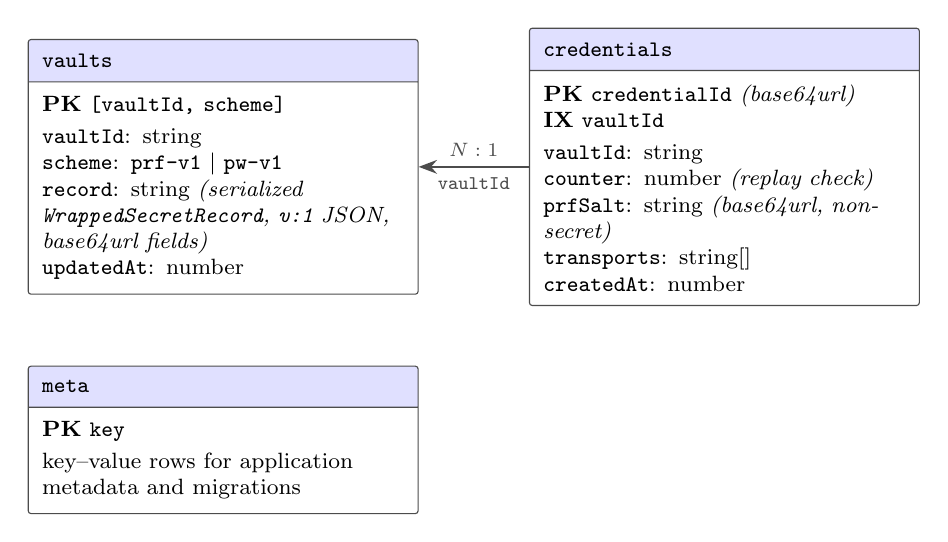
\begin{tikzpicture}[
    font=\footnotesize,
    store/.style={
      rectangle split, rectangle split parts=2, rectangle split part fill={blue!12, white},
      draw=black!70, rounded corners=1pt, align=left, inner sep=5pt,
      text width=4.6cm
    },
    pk/.style={font=\footnotesize\bfseries},
    rel/.style={-{Stealth}, thick, black!70}
  ]
    \node[store] (vaults) {%
      \textbf{\texttt{vaults}}
      \nodepart{two}%
      \textbf{PK} \texttt{[vaultId, scheme]}\\[2pt]
      \texttt{vaultId}: string\\
      \texttt{scheme}: \texttt{prf-v1} $\mid$ \texttt{pw-v1}\\
      \texttt{record}: string \textit{(serialized \texttt{WrappedSecretRecord}, \texttt{v:1} JSON, base64url fields)}\\
      \texttt{updatedAt}: number
    };
    \node[store, right=1.4cm of vaults] (credentials) {%
      \textbf{\texttt{credentials}}
      \nodepart{two}%
      \textbf{PK} \texttt{credentialId} \textit{(base64url)}\\
      \textbf{IX} \texttt{vaultId}\\[2pt]
      \texttt{vaultId}: string\\
      \texttt{counter}: number \textit{(replay check)}\\
      \texttt{prfSalt}: string \textit{(base64url, non-secret)}\\
      \texttt{transports}: string[]\\
      \texttt{createdAt}: number
    };
    \node[store, below=0.9cm of vaults, text width=4.6cm] (meta) {%
      \textbf{\texttt{meta}}
      \nodepart{two}%
      \textbf{PK} \texttt{key}\\[2pt]
      key--value rows for application metadata and migrations
    };
    \draw[rel] (credentials.west) -- node[above, font=\scriptsize]{$N : 1$}
      node[below, font=\scriptsize]{\texttt{vaultId}} (vaults.east);
  \end{tikzpicture}
  \caption{IndexedDB schema created by \texttt{openVaultDb} (database \texttt{zktv}, version~1; \texttt{src/indexeddb/db.ts}). One vault may hold up to two wrapped records (\texttt{prf-v1} and the \texttt{pw-v1} fallback) via the composite primary key, and any number of PRF credentials via the \texttt{vaultId} index. Only wrapped records and non-secret credential metadata are ever persisted.}
  \label{fig:indexeddb-schema}
\end{figure}

\subsection{Migrations and Security Properties}
\texttt{openVaultDb} accepts an \texttt{onUpgrade(db, oldVersion, tx)} hook that runs inside \texttt{onupgradeneeded} \emph{after} the built-in stores are ensured, letting applications version their own stores without touching the core schema. The migration invariant is that no upgrade may introduce stored recomputable key inputs: only \texttt{WrappedSecretRecord} shapes and non-secret credential metadata are ever persisted.
Lifecycle operations preserve this: \texttt{clearVault} deletes both scheme rows for a vault and every credential row bound to it via the \texttt{vaultId} index, and \texttt{securityWipe} clears all three stores (mirroring TrustVault's security-wipe semantics).
Key hygiene throughout: all derived and imported keys are non-extractable \texttt{CryptoKey}s, transient buffers are zeroized in \texttt{finally} blocks, and the signature counter persisted in \texttt{credentials} is updated after each verified assertion (\texttt{updateCounter}) to feed the replay check of Algorithm~\ref{alg:unwrap}.

\section{Implementation in \texttt{webauthn-prf-zktv}}
The library~\cite{zktv-lib} is strict-mode TypeScript, ESM-only, with \texttt{@noble/hashes} (scrypt) as its sole runtime dependency; all other cryptography uses the Web Crypto API.
It ships three sub-path entry points:
\begin{itemize}
  \item \texttt{webauthn-prf-zktv} (core; Node $\geq$20 and browsers): the wrap and unwrap functions of Sect.~4, HKDF and scrypt derivation, record (de)serialization with structural validation, the TrustVault migration adapter, and a typed error hierarchy (\texttt{ZktvError}) whose codes distinguish PRF unavailability, cancelled ceremonies, missing PRF results, replay anomalies, decryption failure, record-format violations, and storage errors.
  \item \texttt{webauthn-prf-zktv/webauthn} (browsers only): capability detection and ceremonies. Detection is deliberately non-invasive. \texttt{detectPrfSupport} is tri-state (supported, unsupported, unknown) via \texttt{getClientCapabilities()} and never creates throwaway credentials to probe; the stricter viability check, \texttt{isPrfViableOnThisClient}, additionally rejects Android WebView --- where PRF does not reach the Credential Manager --- and requires a user-verifying platform authenticator. Enrollment is \emph{adaptive}: \texttt{enrollPrfCredential} requests \texttt{prf.eval} at creation time, so clients that evaluate PRF during registration (e.g.\ recent Chrome with Windows Hello) enroll in a single ceremony; otherwise it hard-verifies \texttt{prf.enabled} in the extension outputs, aborting cleanly if absent, and runs one assertion ceremony to obtain the PRF output. \texttt{evaluatePrf} enforces the 32-byte PRF result length and performs the replay verification of Algorithm~\ref{alg:unwrap}; \texttt{enrollVault} and \texttt{unlockVault} compose ceremony, derivation, and (un)wrapping into single calls that zeroize the PRF output in \texttt{finally} blocks.
  \item \texttt{webauthn-prf-zktv/indexeddb} (browsers only): the \texttt{ZktvDb} storage layer of Sect.~\ref{sec:idb} (Fig.~\ref{fig:indexeddb-schema}).
\end{itemize}

The public API is exercised by unit tests covering the failure paths of Sect.~4 (wrong key, malformed records, replayed assertions) alongside the success paths.
The core wrap entry point, verbatim from \texttt{src/core/wrap.ts}:

\begin{lstlisting}[caption={\texttt{wrapSecret}: the three wrap paths (PRF, password, caller-supplied wrap key).}]
export async function wrapSecret(options: WrapOptions): Promise<WrappedSecretRecord> {
  if ('prfOutput' in options) {
    const wrapKey = await deriveWrapKeyFromPrf(options.prfOutput);
    return encryptRecord(wrapKey, 'prf-v1', options.prfSalt, options.secret);
  }
  if ('password' in options) {
    const salt = options.salt ?? generateSalt();
    const kdfParams = options.kdfParams ?? DEFAULT_SCRYPT_PARAMS;
    const wrapKey = await deriveWrapKeyFromPassword(options.password, salt, kdfParams);
    const record = await encryptRecord(wrapKey, 'pw-v1', salt, options.secret);
    return { ...record, kdfParams };
  }
  return encryptRecord(options.wrapKey, options.scheme, options.salt, options.secret);
}
\end{lstlisting}

\begin{lstlisting}[caption={HKDF derivation with the frozen v1 domain-separation label (\texttt{src/core/derive.ts}).}]
export const HKDF_INFO_V1 = new TextEncoder().encode(
  'webauthn-prf-zktv vault key wrap v1',
);

export async function deriveWrapKeyFromPrf(prfOutput, info = HKDF_INFO_V1) {
  const ikm = await crypto.subtle.importKey('raw', prfOutput, 'HKDF', false, ['deriveKey']);
  return crypto.subtle.deriveKey(
    { name: 'HKDF', hash: 'SHA-256', salt: new Uint8Array(0), info },
    ikm,
    { name: 'AES-GCM', length: 256 },
    false, // non-extractable
    ['encrypt', 'decrypt'],
  );
}
\end{lstlisting}

\section{Post-Quantum Considerations}
\label{sec:pq}
The storage layer of this architecture is built entirely from symmetric primitives --- HMAC-SHA-256 (inside the authenticator PRF), HKDF-SHA256, scrypt, and AES-256-GCM.
Against a quantum adversary, Grover-type speedups at most halve the effective security exponent, leaving AES-256 and SHA-256-based constructions with comfortable margins; NIST's transition guidance accordingly treats AES-256 and SHA-256/384 as quantum-adequate~\cite{nist-pqc}.
Harvest-now, decrypt-later attacks against a captured IndexedDB dump are therefore not materially assisted by future quantum capability.

The asymmetric layer is different: today's passkeys sign with elliptic-curve or RSA algorithms (the library requests ES256 and RS256), which fall to a cryptographically relevant quantum computer.
However, that layer protects \emph{authentication}, not the confidentiality of stored records: breaking the signature scheme lets an attacker forge assertions toward a relying party, but does not reveal the \texttt{hmac-secret} key inside the authenticator, and hence not the PRF output or $K_v$.
Because the wrapping scheme is agnostic to the credential's signature algorithm, PQ-capable passkeys (e.g.\ ML-DSA-based, as they appear in authenticators) can be adopted without any change to the record format; a future \texttt{prf-v2} scheme identifier is reserved for the case where the KDF or cipher itself must move.

\section{Evaluation and Discussion}
The reference implementation is evaluated along three axes.
\emph{Security}: the zero-knowledge argument of Sect.~\ref{sec:zk} covers the persisted state; the unit-test suite additionally pins the negative behaviors the argument relies on --- wrong-key decryption is indistinguishable from corruption, malformed records never reach the cipher, and non-increasing signature counters abort the unlock.
\emph{Performance}: unlock cost is dominated by the WebAuthn ceremony itself (user verification takes seconds), against which one HKDF derivation and one AES-GCM decryption of a 32-byte payload are negligible; on the password fallback path, scrypt with $N{=}2^{17}$ deliberately costs a few hundred milliseconds on commodity hardware, a floor chosen so that offline guessing, not interactive unlock, bears the cost.
\emph{Usability}: PRF-based unlock replaces master-password entry with a platform biometric gesture, but availability is uneven across browsers, platforms, and embedded WebViews; the tri-state capability detection and the \texttt{pw-v1} fallback exist precisely so that applications degrade gracefully rather than probe destructively.
A quantitative cross-device benchmark of ceremony latency and PRF availability is left as future work.

\section{Conclusion}
This paper formalized a WebAuthn PRF-based vault key wrapping scheme --- PRF output as HKDF input keying material under a frozen, versioned domain-separation label, wrapping a non-extractable AES-256-GCM vault key --- together with an IndexedDB storage architecture whose entire persisted state provably contains no recomputable key inputs.
The scheme integrates client-side replay verification, a memory-hard password fallback for clients where PRF is unavailable, and a ceremony-free migration path from the predecessor TrustVault-PWA format.
The open-source \texttt{webauthn-prf-zktv} library~\cite{zktv-lib} packages these patterns behind small, typed entry points so that other web applications can adopt PRF-based zero-knowledge vaults without re-deriving the storage and key-hygiene discipline described here.

\bibliographystyle{plain}
\bibliography{references}

\end{document}
